\documentclass[]{article}
\usepackage{lmodern}
\usepackage{amssymb,amsmath}
\usepackage{ifxetex,ifluatex}
\usepackage{fixltx2e} % provides \textsubscript
\ifnum 0\ifxetex 1\fi\ifluatex 1\fi=0 % if pdftex
  \usepackage[T1]{fontenc}
  \usepackage[utf8]{inputenc}
\else % if luatex or xelatex
  \ifxetex
    \usepackage{mathspec}
  \else
    \usepackage{fontspec}
  \fi
  \defaultfontfeatures{Ligatures=TeX,Scale=MatchLowercase}
\fi
% use upquote if available, for straight quotes in verbatim environments
\IfFileExists{upquote.sty}{\usepackage{upquote}}{}
% use microtype if available
\IfFileExists{microtype.sty}{%
\usepackage[]{microtype}
\UseMicrotypeSet[protrusion]{basicmath} % disable protrusion for tt fonts
}{}
\PassOptionsToPackage{hyphens}{url} % url is loaded by hyperref
\usepackage[unicode=true]{hyperref}
\hypersetup{
            pdfborder={0 0 0},
            breaklinks=true}
\urlstyle{same}  % don't use monospace font for urls
\usepackage{color}
\usepackage{fancyvrb}
\newcommand{\VerbBar}{|}
\newcommand{\VERB}{\Verb[commandchars=\\\{\}]}
\DefineVerbatimEnvironment{Highlighting}{Verbatim}{commandchars=\\\{\}}
% Add ',fontsize=\small' for more characters per line
\newenvironment{Shaded}{}{}
\newcommand{\KeywordTok}[1]{\textcolor[rgb]{0.00,0.44,0.13}{\textbf{#1}}}
\newcommand{\DataTypeTok}[1]{\textcolor[rgb]{0.56,0.13,0.00}{#1}}
\newcommand{\DecValTok}[1]{\textcolor[rgb]{0.25,0.63,0.44}{#1}}
\newcommand{\BaseNTok}[1]{\textcolor[rgb]{0.25,0.63,0.44}{#1}}
\newcommand{\FloatTok}[1]{\textcolor[rgb]{0.25,0.63,0.44}{#1}}
\newcommand{\ConstantTok}[1]{\textcolor[rgb]{0.53,0.00,0.00}{#1}}
\newcommand{\CharTok}[1]{\textcolor[rgb]{0.25,0.44,0.63}{#1}}
\newcommand{\SpecialCharTok}[1]{\textcolor[rgb]{0.25,0.44,0.63}{#1}}
\newcommand{\StringTok}[1]{\textcolor[rgb]{0.25,0.44,0.63}{#1}}
\newcommand{\VerbatimStringTok}[1]{\textcolor[rgb]{0.25,0.44,0.63}{#1}}
\newcommand{\SpecialStringTok}[1]{\textcolor[rgb]{0.73,0.40,0.53}{#1}}
\newcommand{\ImportTok}[1]{#1}
\newcommand{\CommentTok}[1]{\textcolor[rgb]{0.38,0.63,0.69}{\textit{#1}}}
\newcommand{\DocumentationTok}[1]{\textcolor[rgb]{0.73,0.13,0.13}{\textit{#1}}}
\newcommand{\AnnotationTok}[1]{\textcolor[rgb]{0.38,0.63,0.69}{\textbf{\textit{#1}}}}
\newcommand{\CommentVarTok}[1]{\textcolor[rgb]{0.38,0.63,0.69}{\textbf{\textit{#1}}}}
\newcommand{\OtherTok}[1]{\textcolor[rgb]{0.00,0.44,0.13}{#1}}
\newcommand{\FunctionTok}[1]{\textcolor[rgb]{0.02,0.16,0.49}{#1}}
\newcommand{\VariableTok}[1]{\textcolor[rgb]{0.10,0.09,0.49}{#1}}
\newcommand{\ControlFlowTok}[1]{\textcolor[rgb]{0.00,0.44,0.13}{\textbf{#1}}}
\newcommand{\OperatorTok}[1]{\textcolor[rgb]{0.40,0.40,0.40}{#1}}
\newcommand{\BuiltInTok}[1]{#1}
\newcommand{\ExtensionTok}[1]{#1}
\newcommand{\PreprocessorTok}[1]{\textcolor[rgb]{0.74,0.48,0.00}{#1}}
\newcommand{\AttributeTok}[1]{\textcolor[rgb]{0.49,0.56,0.16}{#1}}
\newcommand{\RegionMarkerTok}[1]{#1}
\newcommand{\InformationTok}[1]{\textcolor[rgb]{0.38,0.63,0.69}{\textbf{\textit{#1}}}}
\newcommand{\WarningTok}[1]{\textcolor[rgb]{0.38,0.63,0.69}{\textbf{\textit{#1}}}}
\newcommand{\AlertTok}[1]{\textcolor[rgb]{1.00,0.00,0.00}{\textbf{#1}}}
\newcommand{\ErrorTok}[1]{\textcolor[rgb]{1.00,0.00,0.00}{\textbf{#1}}}
\newcommand{\NormalTok}[1]{#1}
\usepackage{graphicx,grffile}
\makeatletter
\def\maxwidth{\ifdim\Gin@nat@width>\linewidth\linewidth\else\Gin@nat@width\fi}
\def\maxheight{\ifdim\Gin@nat@height>\textheight\textheight\else\Gin@nat@height\fi}
\makeatother
% Scale images if necessary, so that they will not overflow the page
% margins by default, and it is still possible to overwrite the defaults
% using explicit options in \includegraphics[width, height, ...]{}
\setkeys{Gin}{width=\maxwidth,height=\maxheight,keepaspectratio}
\IfFileExists{parskip.sty}{%
\usepackage{parskip}
}{% else
\setlength{\parindent}{0pt}
\setlength{\parskip}{6pt plus 2pt minus 1pt}
}
\setlength{\emergencystretch}{3em}  % prevent overfull lines
\providecommand{\tightlist}{%
  \setlength{\itemsep}{0pt}\setlength{\parskip}{0pt}}
\setcounter{secnumdepth}{0}
% Redefines (sub)paragraphs to behave more like sections
\ifx\paragraph\undefined\else
\let\oldparagraph\paragraph
\renewcommand{\paragraph}[1]{\oldparagraph{#1}\mbox{}}
\fi
\ifx\subparagraph\undefined\else
\let\oldsubparagraph\subparagraph
\renewcommand{\subparagraph}[1]{\oldsubparagraph{#1}\mbox{}}
\fi

% set default figure placement to htbp
\makeatletter
\def\fps@figure{htbp}
\makeatother


\date{}

\begin{document}

SiScLab 2018 Student Project \textbf{Analysis Tool for Materials
Design}. Written in Python3.

Authors: \href{https://github.com/Irratzo}{Johannes Wasmer},
\href{https://github.com/ChristianPartmann}{Christian Partmann}, and
\href{https://github.com/PraneethKatta}{Praneeth Katta}.

\section{Overview}\label{overview}

This subfolder \texttt{studentproject18ws} is currently a largely
independent side-project accompanying the main module
\texttt{masci-tools}. It was created in a student project, and consists
of three submodules:

\begin{itemize}
\tightlist
\item
  preprocessor: a HDF reader interface, and one implementation for Fleur
  band structure simulation output
\item
  visualization: a plotting interface, and one implementation for Fleur
  bandstructure+DOS plots
\item
  frontends: a Desktop GUI and a Web Dashboard (Tk and Jupyter) for
  interactive Fleur bandDOS plots.
\end{itemize}

A more thorough description and example use cases can be found in the
project \href{./doc/report.pdf}{report} and
\href{./doc/presentation.pdf}{presentation}.

\begin{figure}
\centering
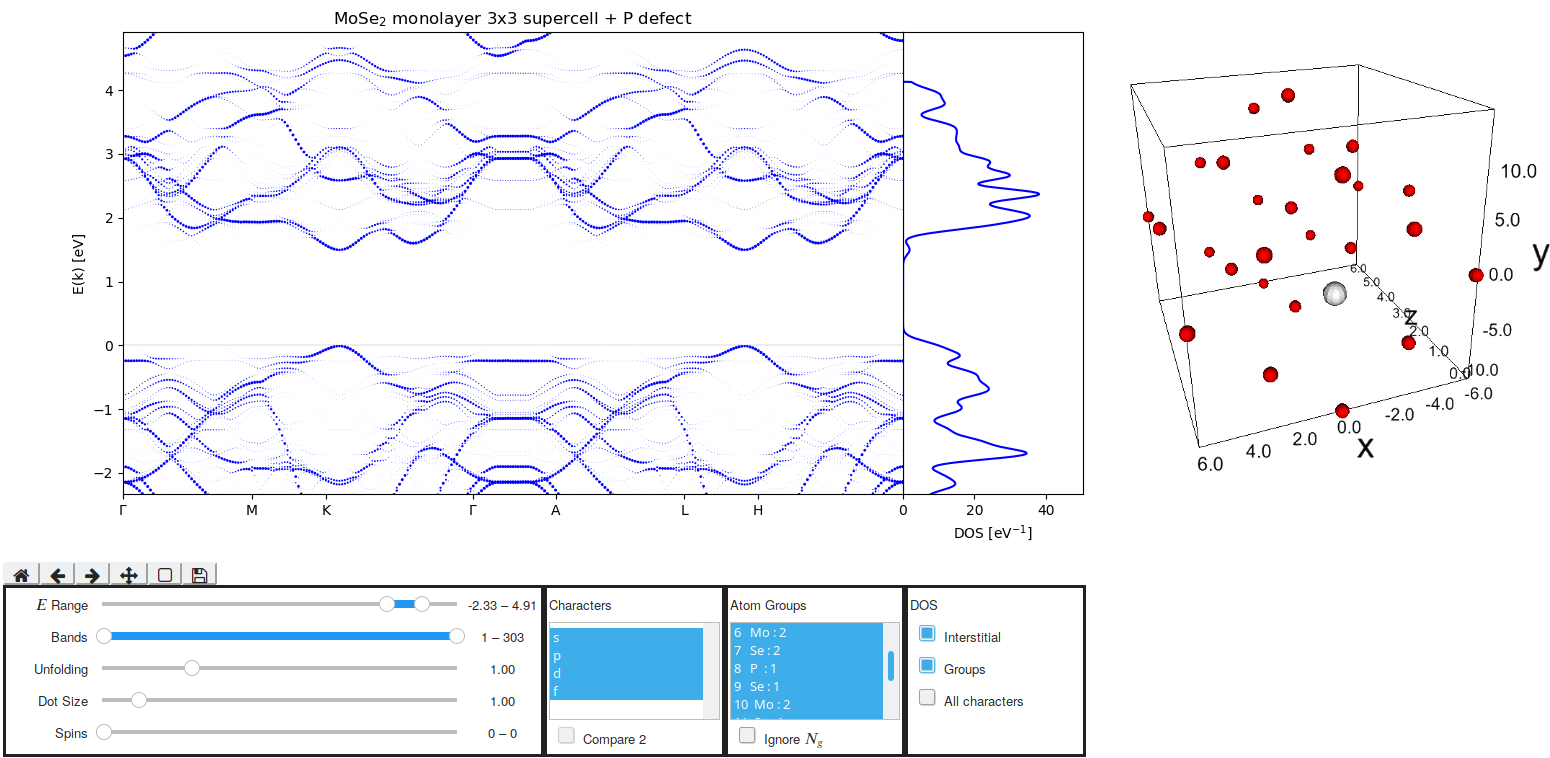
\includegraphics{./readme/web_frontend.png}
\caption{}
\end{figure}

\section{For Frontend Users}\label{for-frontend-users}

The Desktop GUI executable can be received from the developers on
request. Otherwise, it can be built using
\href{https://www.pyinstaller.org/}{PyInstaller} from this repo.

The Web Frontend is a Jupyter Dashboard. It is in experimental phase (no
fileupload yet). You can try it out
\href{https://mybinder.org/v2/gh/JuDFTteam/masci-tools/studentproject18ws?filepath=studentproject18w\%2Ffrontend\%2Fjupyter\%2Fdemo\%2Fbinder_demo.ipynb}{here
on Binder}. You can run it locally (see developer section). If you have
an \href{https://aiidalab.materialscloud.org/hub/login}{AiiDaLab
account}: the dashboard is planned to be published as an app there.

\section{For Developers}\label{for-developers}

\subsection{Installation}\label{installation}

Though \texttt{masci-tools} is availabe via PyPI, there is currently no
plan to integrate \texttt{studentproject18ws}. If you want to use it in
your code, clone the repo, use it in an IDE, or append the path to your
\texttt{sys.path}:

\begin{Shaded}
\begin{Highlighting}[]
\ImportTok{import}\NormalTok{ sys}
\ControlFlowTok{if}\NormalTok{ path_repo }\KeywordTok{not} \KeywordTok{in}\NormalTok{ sys.path:}
\NormalTok{    sys.path.append(path_repo)}
    
\CommentTok{# now import works}
\ImportTok{from}\NormalTok{ studentproject18w.hdf.reader }\ImportTok{import}\NormalTok{ Reader}
\CommentTok{# ...}
\end{Highlighting}
\end{Shaded}

\subsubsection{Create project virtual
environment}\label{create-project-virtual-environment}

With conda (recommended): -
\href{https://www.anaconda.com/download}{Install Anaconda (3
recommended)} - Install the environment \texttt{masci-stupro} with the
necessary and recommended dependencies:

\begin{Shaded}
\begin{Highlighting}[]
\ExtensionTok{conda}\NormalTok{ create -f environment.yml}
\BuiltInTok{source}\NormalTok{ activate masci-stupro}
\end{Highlighting}
\end{Shaded}

With virtualenv (untested):

\begin{Shaded}
\begin{Highlighting}[]
\ExtensionTok{virtualenv}\NormalTok{ masci-stupro}
\BuiltInTok{source}\NormalTok{ masci-stupro/bin/activate}
\ExtensionTok{pip}\NormalTok{ install -r requirements_pip.txt }\CommentTok{# install requirements}
\end{Highlighting}
\end{Shaded}

\subsection{Programmatic use}\label{programmatic-use}

In this example, a Fleur HDF file is preprocessed using the Recipe
\texttt{FleurBands}. The resulting output \texttt{data} is then passed
to a plotter, alongside some DOS CSV files for a bandstructure plot
using \texttt{matplotlib} as backend library.

\begin{Shaded}
\begin{Highlighting}[]
\ImportTok{import}\NormalTok{ matplotlib.pyplot }\ImportTok{as}\NormalTok{ plt}
\ImportTok{from}\NormalTok{ studentproject18w.hdf.reader }\ImportTok{import}\NormalTok{ Reader}
\ImportTok{from}\NormalTok{ studentproject18w.hdf.recipes }\ImportTok{import}\NormalTok{ Recipes}
\ImportTok{from}\NormalTok{ studentproject18w.plot.matplot }\ImportTok{import}\NormalTok{ BandDOSPlot}

\NormalTok{data }\OperatorTok{=} \VariableTok{None}
\NormalTok{reader }\OperatorTok{=}\NormalTok{ Reader(filepath}\OperatorTok{=}\NormalTok{filepath_hdf)}
\ControlFlowTok{with}\NormalTok{ reader }\ImportTok{as}\NormalTok{ h5file:}
\NormalTok{    data }\OperatorTok{=}\NormalTok{ reader.read(recipe}\OperatorTok{=}\NormalTok{Recipes.FleurBands)}
    \CommentTok{#}
    \CommentTok{# Note:}
    \CommentTok{# Inside the with statement (context manager),}
    \CommentTok{# all data attributes that are type h5py Dataset are available (in-file access)}
    \CommentTok{# When the statement is left,the HDF5 file gets closed and the datasets are closed.}
    \CommentTok{#}
    \CommentTok{# Use data outside the with-statement (in-memory access: all HDF5 datasets converted to numpy ndarrays):}
\NormalTok{    data.move_datasets_to_memory()}

\NormalTok{plotter }\OperatorTok{=}\NormalTok{ BandDOSPlot(plt, data, filepaths_dos)}
\NormalTok{(fig, ax_bands, ax_dos) }\OperatorTok{=}\NormalTok{ plter.setup_figure(fig_ratio}\OperatorTok{=}\NormalTok{[}\DecValTok{12}\NormalTok{,}\DecValTok{6}\NormalTok{], fig_scale}\OperatorTok{=}\DecValTok{1}\NormalTok{, fig_title}\OperatorTok{=}\StringTok{"BandDOS"}\NormalTok{)}
\NormalTok{data_selection }\OperatorTok{=}\NormalTok{ make_selection()}
\NormalTok{plotter.plot_bandDOS(}\OperatorTok{*}\NormalTok{data_selection)}
\NormalTok{plt.show()}
\end{Highlighting}
\end{Shaded}

\subsection{Try out Web Frontend
locally}\label{try-out-web-frontend-locally}

The demo notebook with the Dashboard is
\texttt{studentproject18w/frontend/jupyter/demo/demo.ipynb}.

\subsubsection{If using Jupyter
Notebook}\label{if-using-jupyter-notebook}

If using Windows, omit keyword \texttt{source}.

\begin{Shaded}
\begin{Highlighting}[]
\BuiltInTok{source}\NormalTok{ activate masci-stupro}
\BuiltInTok{cd}\NormalTok{ mypath/masci-tools/studentproject18ws/}
\ExtensionTok{jupyter-notebook}\NormalTok{ .}
\CommentTok{# if Home is not set to this dir, try this instead:}
\CommentTok{# /home/you/anaconda3/envs/myenv/bin/python /home/you/anaconda3/envs/myenv/bin/jupyter-notebook .}
\end{Highlighting}
\end{Shaded}

\subsubsection{If using Jupyter Lab}\label{if-using-jupyter-lab}

Additional installation step needed:
`\texttt{bash\ source\ activate\ masci-stupro\ jupyter\ labextension\ install\ @jupyter-widgets/jupyterlab-manager\ jupyter-matplotlib\ ipyvolume\ cd\ mypath/masci-tools/studentproject18ws/\ jupyter-lab}**

\subsection{To-do list for publishing the Web
Frontend}\label{to-do-list-for-publishing-the-web-frontend}

\begin{itemize}
\tightlist
\item
  (recommended: create \texttt{frontend/jupyter/Dashboard.py} widget and
  put code of
  \href{./frontend/jupyter/demo/demo_backend.ipynb}{demo\_back.ipynb}
  notebook inside it. Use
  \href{https://github.com/aiidalab/aiidalab-widgets-base/blob/master/aiidalab_widgets_base/structures.py}{aiidalab-widgets-base
  \textgreater{} StructureUploadWidget} as a template. Create
  \texttt{frontend/jupyter/Dashboard.ipynb} notebook. Use
  \href{https://github.com/aiidalab/aiidalab-widgets-base/blob/master/structures.ipynb}{StructureUploadWidget
  Demo Notebook} as a template.)
\item
  Add \href{https://pypi.org/project/fileupload/}{fileupload} to widget
  (again, like in StructureUploadWidget. See
  \href{./frontend/jupyter/demo/binder_fileupload_test.ipynb}{binder\_fileupload\_test.ipynb}
  notebook for a demo that works with binder.)
\item
  Now the Web Frontend should work on Binder.
\item
  For publishing the app on AiiDA Lab, the app has to be registered in
  the
  \href{https://github.com/aiidalab/aiidalab-registry}{aiidalab-registry}.

  \begin{itemize}
  \tightlist
  \item
    The project code is in Python3, but aiidalab requires Python2. So
    the code has to first be backported by hand using the
    \texttt{future} package. If this takes too long, maybe try the tool
    \href{https://pypi.org/project/3to2/}{3to2}.
  \item
    Use the simplest app in the registry,
    \href{https://github.com/aiidalab/aiidalab-units}{aiidalab-units} as
    a template. Adapt code.
  \item
    Try it out first in the
    \href{https://www.materialscloud.org/work/quantum-mobile}{Quantum
    Mobile Virtual Machine}, which has aiidalab installed and
    configured. Else try it in a virtual environment with
    \href{https://pypi.org/project/aiidalab/}{aiidalab} installed from
    PyPI.
  \item
    Register the app.
  \end{itemize}
\end{itemize}

Note: other publishing options besides Binder and AiiDALab are listed
\href{https://github.com/markusschanta/awesome-jupyter}{here}. For
instance, \href{http://colab.research.google.com/}{Google Colaboratory}
is a free Notebook hosting service that allows file upload.

\end{document}
